\documentclass[11pt]{article}
\usepackage{listings}
\usepackage[letterpaper]{geometry}
\usepackage{float}
\usepackage{graphicx}
\graphicspath{{./images/}}

\begin{document}

Morgan Rosenkranz 
EECE5644 
5/2/21 

\section*{Question 1:}
I began by generating training data sets of 20, 200, and 2000 samples and a validation set of 10000 samples.
To create the two classes I used the given means and covariances and generated a mixed Gaussian as specified by the problem and weights.

\subsection*{Part 1:}
Using the given means and covariances I created a theoretically optimal classifier and applied it to the validation dataset.
I then varied the threshold which gave the following ROC curve.

\begin{figure}[H]
	\centering
	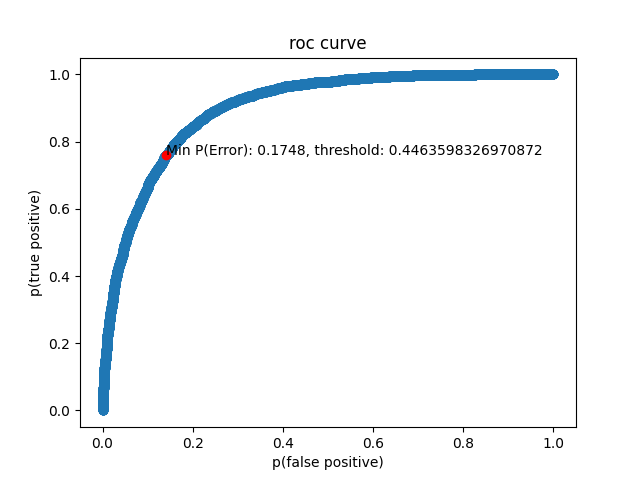
\includegraphics[width=0.75\textwidth]{optimal_roc}
	\caption{ROC Curve With Optimal Classifier}
\end{figure}

The threshold for which the minimum probability of error was reached is 0.44 while the minimum probability of error is 0.174.
This point is marked on the ROC curve in red.

Using this optimal threshold I then recategorized the data in the validation set and plotted the original and estimated classes side by side:

\begin{figure}[H]
	\centering
	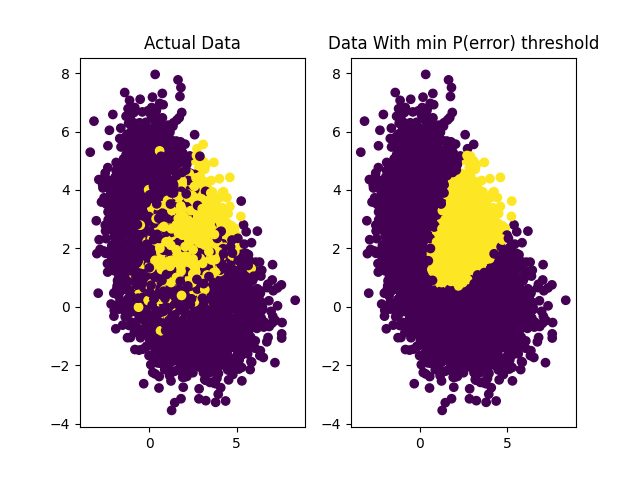
\includegraphics[width=0.75\textwidth]{optimal_data}
	\caption{Actual Data Comparison to Optimal Classifier}
\end{figure}

This gave a pretty good estimate but some of the mixture is clearly lost in the boundary.

\subsection*{Part 2:}
Using the three training datasets from earlier I created a linear and quadratic function based approximations of class labels.

For the linear case I used the function:

\[
	h(x,w) = \frac{1}{1 + e^{-w^T [1,x^T]^T}}
\]

I then used the scipy Nelder-Mead minimize function to find the w vector which minimized the cost of the line drawn between class groups,
effectively finding the w with the best fit to the data.

This resulted in the following division of the class labels:

\begin{figure}[H]
	\centering
	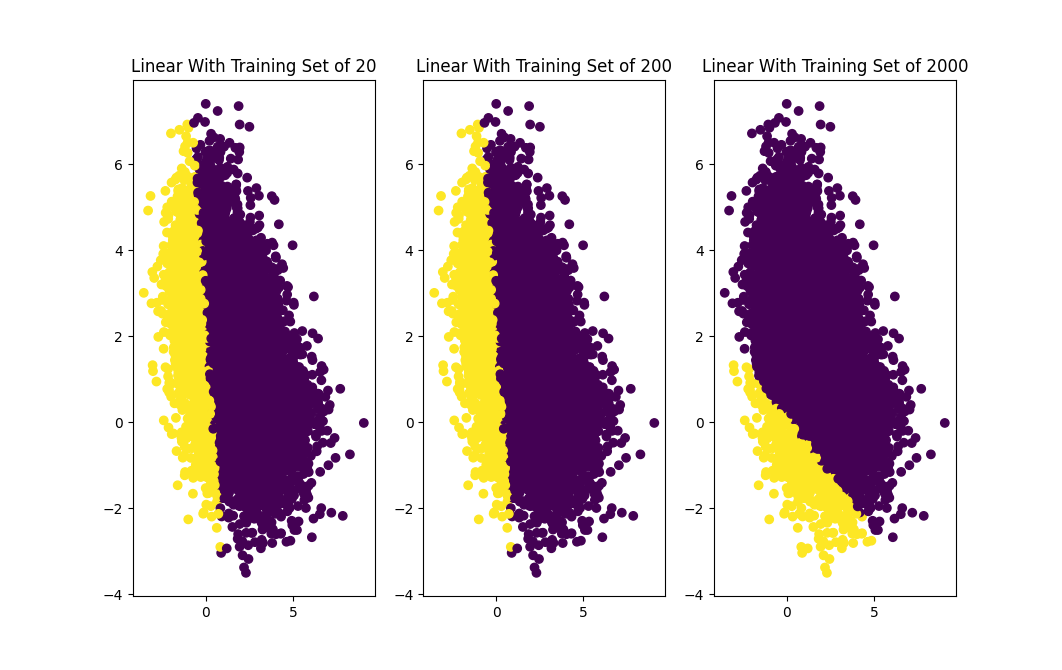
\includegraphics[width=1.0\textwidth]{linear_data}
	\caption{Results of Linear Classifier}
\end{figure}

The linear classifier does not compare at all to the ability of the optimal classifier.
The line bisects the dataset and does not do well in the nuances of categorizing the mixture.

For the quadratic case I used the function:
\[
	h(x,w) = \frac{1}{1 + e^{-w^T [1,x_1,x_2,x_1^2,x_1x_2,x_2^2]^T}}
\]

I then used the same methods as above the train the function with the different training sets and applied them to the validation set.

\begin{figure}[H]
	\centering
	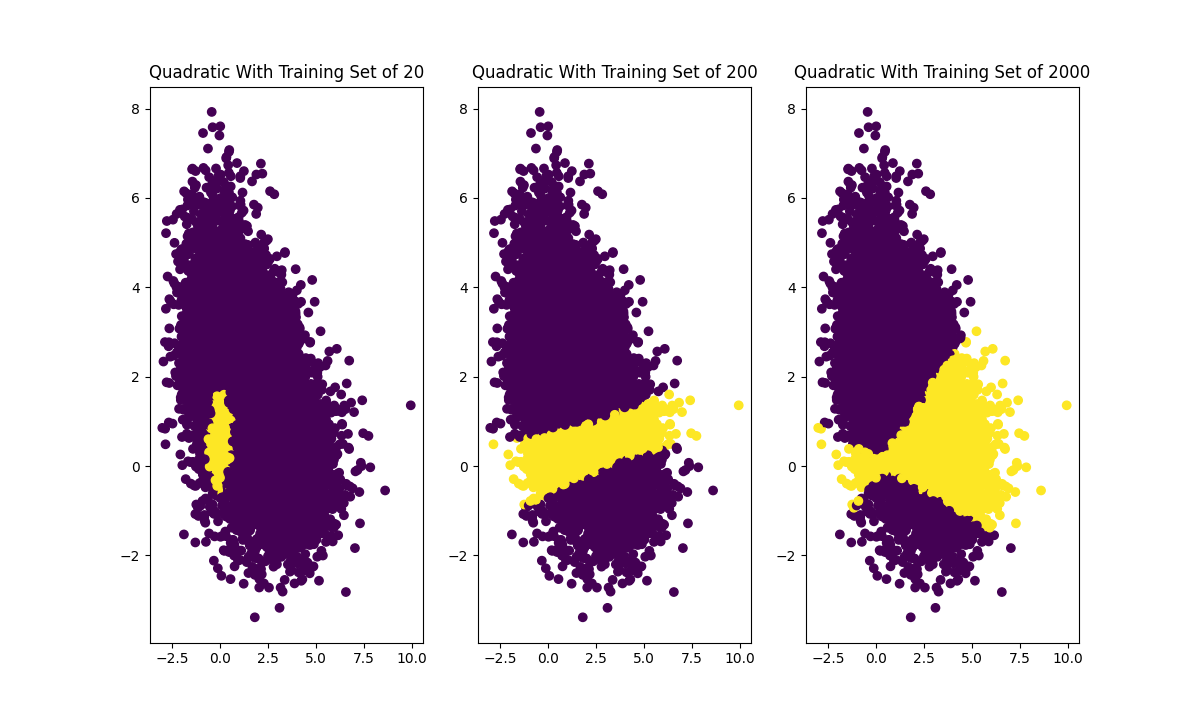
\includegraphics[width=1.0\textwidth]{quad_data}
	\caption{Results of Linear Classifier}
\end{figure}

The quad classifier performed much better than the linear but still was not close to the performance of the optimal.

\section*{Question 2:}
For this question I used the provided code to generate a training and validation data set for a maximum likelihood estimator and a MAP estimator.
For the ML estimator I used the following equation to estimate w:
\[
	w = [\frac{1}{N}\sum_{i=1}^{N}Z_iZ_i^T + \gamma I]^{-1} \frac{1}{N}\sum_{i=1}^{N}y_iZ_i
\]

For the MAP estimator I used the following equation to estimate w:
\[
	w = [\frac{1}{N}\sum_{i=1}^{N}Z_iZ_i^T]^{-1} \frac{1}{N}\sum_{i=1}^{N}y_iZ_i
\]

I then varied gamma from $10^-4$ to $10^7$ and calculated the average squared distance for all gamma values and plotted them below:

\begin{figure}[H]
	\centering
	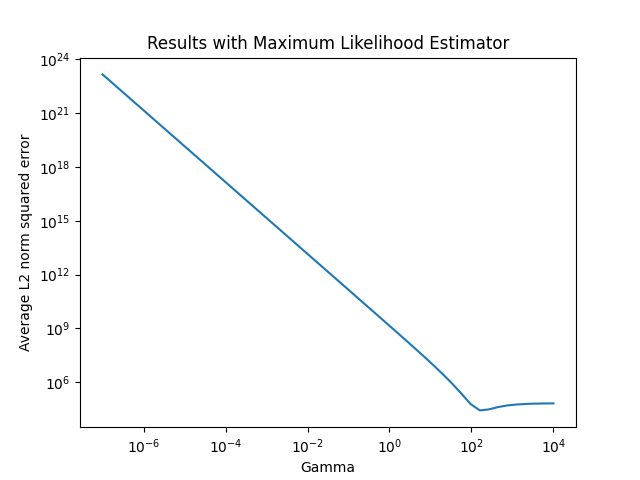
\includegraphics[width=0.75\textwidth]{ml_gamma}
	\caption{Gamma vs. Error for ML}
\end{figure}

\begin{figure}[H]
	\centering
	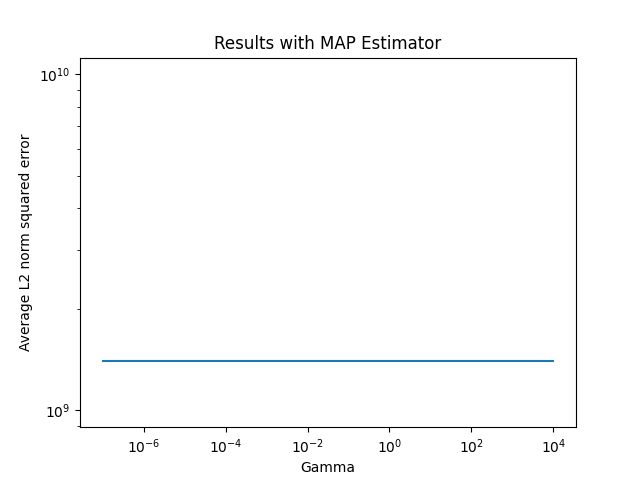
\includegraphics[width=0.75\textwidth]{map_gamma}
	\caption{Gamma vs. Error for MAP}
\end{figure}

Below I compare the original data set, ML estimated, and MAP estimated, all on the validation data set.

\begin{figure}[H]
	\centering
	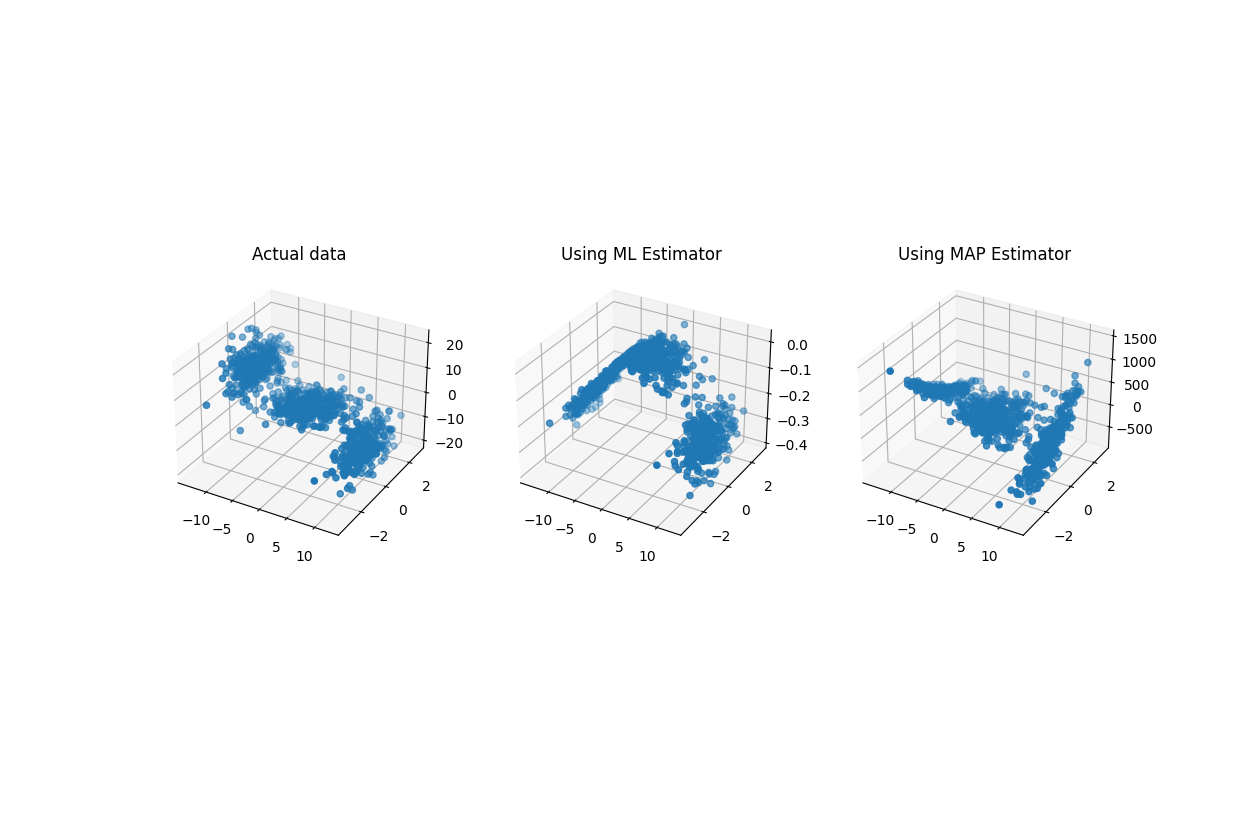
\includegraphics[width=1.0\textwidth]{comparison}
	\caption{Comparison of Actual and Estimated Datasets}
\end{figure}

Neither performed particularly well but the ML version had a minimum error that is significantly lower than the MAP.
MAP estimator did not vary it's error with different gammas which is likely due to the equations used for calculating w.
One can see that the generated w's do create variation in y but not exactly the kind we want.
The ML estimator seems to have settled on creating a parabola while the MAP estimator seems to have skewed the results in relation to $x_2$.
I would say that the ML estimator appears to have done a better job with the first and last Gaussian distributions but failed to approximate the middle.
The MAP estimator predicted each group but with seemingly equal amounts of error in their distributions.

\subsection*{Part 3:}

\subsection*{ML Estimator for $\Theta$}
First I set up the maximum likelihood estimator for $\Theta$:
\[
	\hat{\Theta}_{ml} = argmax_{\theta} \sum_{i=1}^{N} \ln p(Z=z_i\vert \theta)
\]

I broke the dataset D into its individual Z elements so that I could do the next step of representing the likelihood in terms of the corresponding $\theta$ for each z.

\[
	\hat{\Theta}_{ml} = argmax_{\theta} \sum_{i=1}^{N} \ln \theta_{z_i}
\]

From here I could create a Lagrange multiplier to find find values for $\Theta$ which satisfy the condition that all probabilities of $\theta_{z_i}$
add up to 1.

\[
	L(\theta, \lambda) = \sum_{i=1}^{N} \ln \theta_{z_i} - \lambda(\sum_{k=1}^{K}\theta_k - 1)
\]

We can then solve for $\Theta$ with the system of equations:

\[
	\frac{\partial L(\theta, \lambda)}{\partial \theta} = 0,
	\frac{\partial L(\theta, \lambda)}{\partial \lambda} = 0 
\]

\subsection*{MAP Estimator for $\Theta$}
The MAP estimator is similar to the ML except we include the prior:

\[
	\hat{\Theta}_{ml} = argmax_{\theta} \sum_{i=1}^{N} \ln \theta_{z_i} + \ln p(\theta)
\]

I then substituted the Dirichlet distribution given for $p(\Theta)$

\[
	\hat{\Theta}_{ml} = argmax_{\theta} \sum_{i=1}^{N} \ln \theta_{z_i}
	+ \ln \frac{\Gamma(\sum_{k=1}^{K} \alpha_k)}{\prod_{k=1}^{K}\Gamma(\alpha_k)} \sum_{k=1}^{K} \theta_k^{\alpha_k -1}
\]

I then used the Lagrange as before, but this time one needs to use the hyper-parameter $\alpha$, maybe using k-fold cross validation.

\section*{Code}
\subsection*{Code for Question 1}
\lstinputlisting[language=python]{q1.py}

\subsection*{Code for Question 2}
\lstinputlisting[language=python]{q2.py}
\end{document}
